\subsection{Architecture}
\subsubsection{Design Overview}
\textbf{VLANs} \\
The upgraded network ensures that departments and specific services are 
isolated (per the new network requirements) by distributing them across 
separate VLANs. This configuration allows for any combination of hosts assigned 
to different departments to be physically attached to the same switch (in the 
event that physical separation is not feasible), while maintaining separation.
\\

\noindent The VLANs are assigned as follows:
\newcolumntype{P}[1]{>{\centering\arraybackslash}p{#1}}
\begin{center}
    \begin{tabular}{|P{2.0cm}|P{1.2cm}|P{4.0cm}|}
    \hline
        \textbf{Addresses} & \textbf{VLAN} & \textbf{Department/Service}\\
    \hline
        10.1.110.0/24 & 10 & Executives \\
    \hline
        10.1.120.0/24 & 20 & Human Resources \\
    \hline
        10.1.130.0/24 & 30 & Research \& Development \\
    \hline
        10.1.140.0/24 & 40 & Engineering \\
    \hline
        10.1.150.0/24 & 50 & Sales \\
    \hline
        10.1.160.0/24 & 60 & Internal Services \\
    \hline
        10.1.170.0/24 & 70 & DMZ \\
    \hline
\end{tabular}
\end{center}

\noindent
\textbf{Inter-Router/Switch Interfaces} \\
Interfaces between router-router and switch-router (and vice versa) are assigned
addresses with a CIDR of /30, and the address space 10.1.2.0/24 is reserved
specifically for these interfaces.  \\

\noindent
\textbf{Switch Ports} \\
Switch ports are statically assigned, as needed, within the address space of 
10.1.10.0/24. \\

\noindent
\textbf{Static Hosts} \\
Special host IP addresses (specific services, such as DHCP, etc.) are 
statically within the address space of 10.1.160.0/24. \\

\noindent
\textbf{Department Hosts} \\
Department host (workstations) IP addresses are dynamically assigned by the DHCP
server. \\

Through our topology we have upgraded from an all layer 2 network to a 
combination of layer 2 and layer 3. Thus allowing for a more robust and "smart" 
network. With the implementation of layer 3 we have added routers to control 
the broadcast signals that were not controlled within the previous network. We 
have added redundancy to the network allowing multiple connection points. To 
control the restrictions we have upgraded the network with VLANs. Thus ensuring 
isolated departments and services by dividing them into separate VLANs. 
 
\subsubsection{Network Topology Map}
\begin{figure}[!htb]
	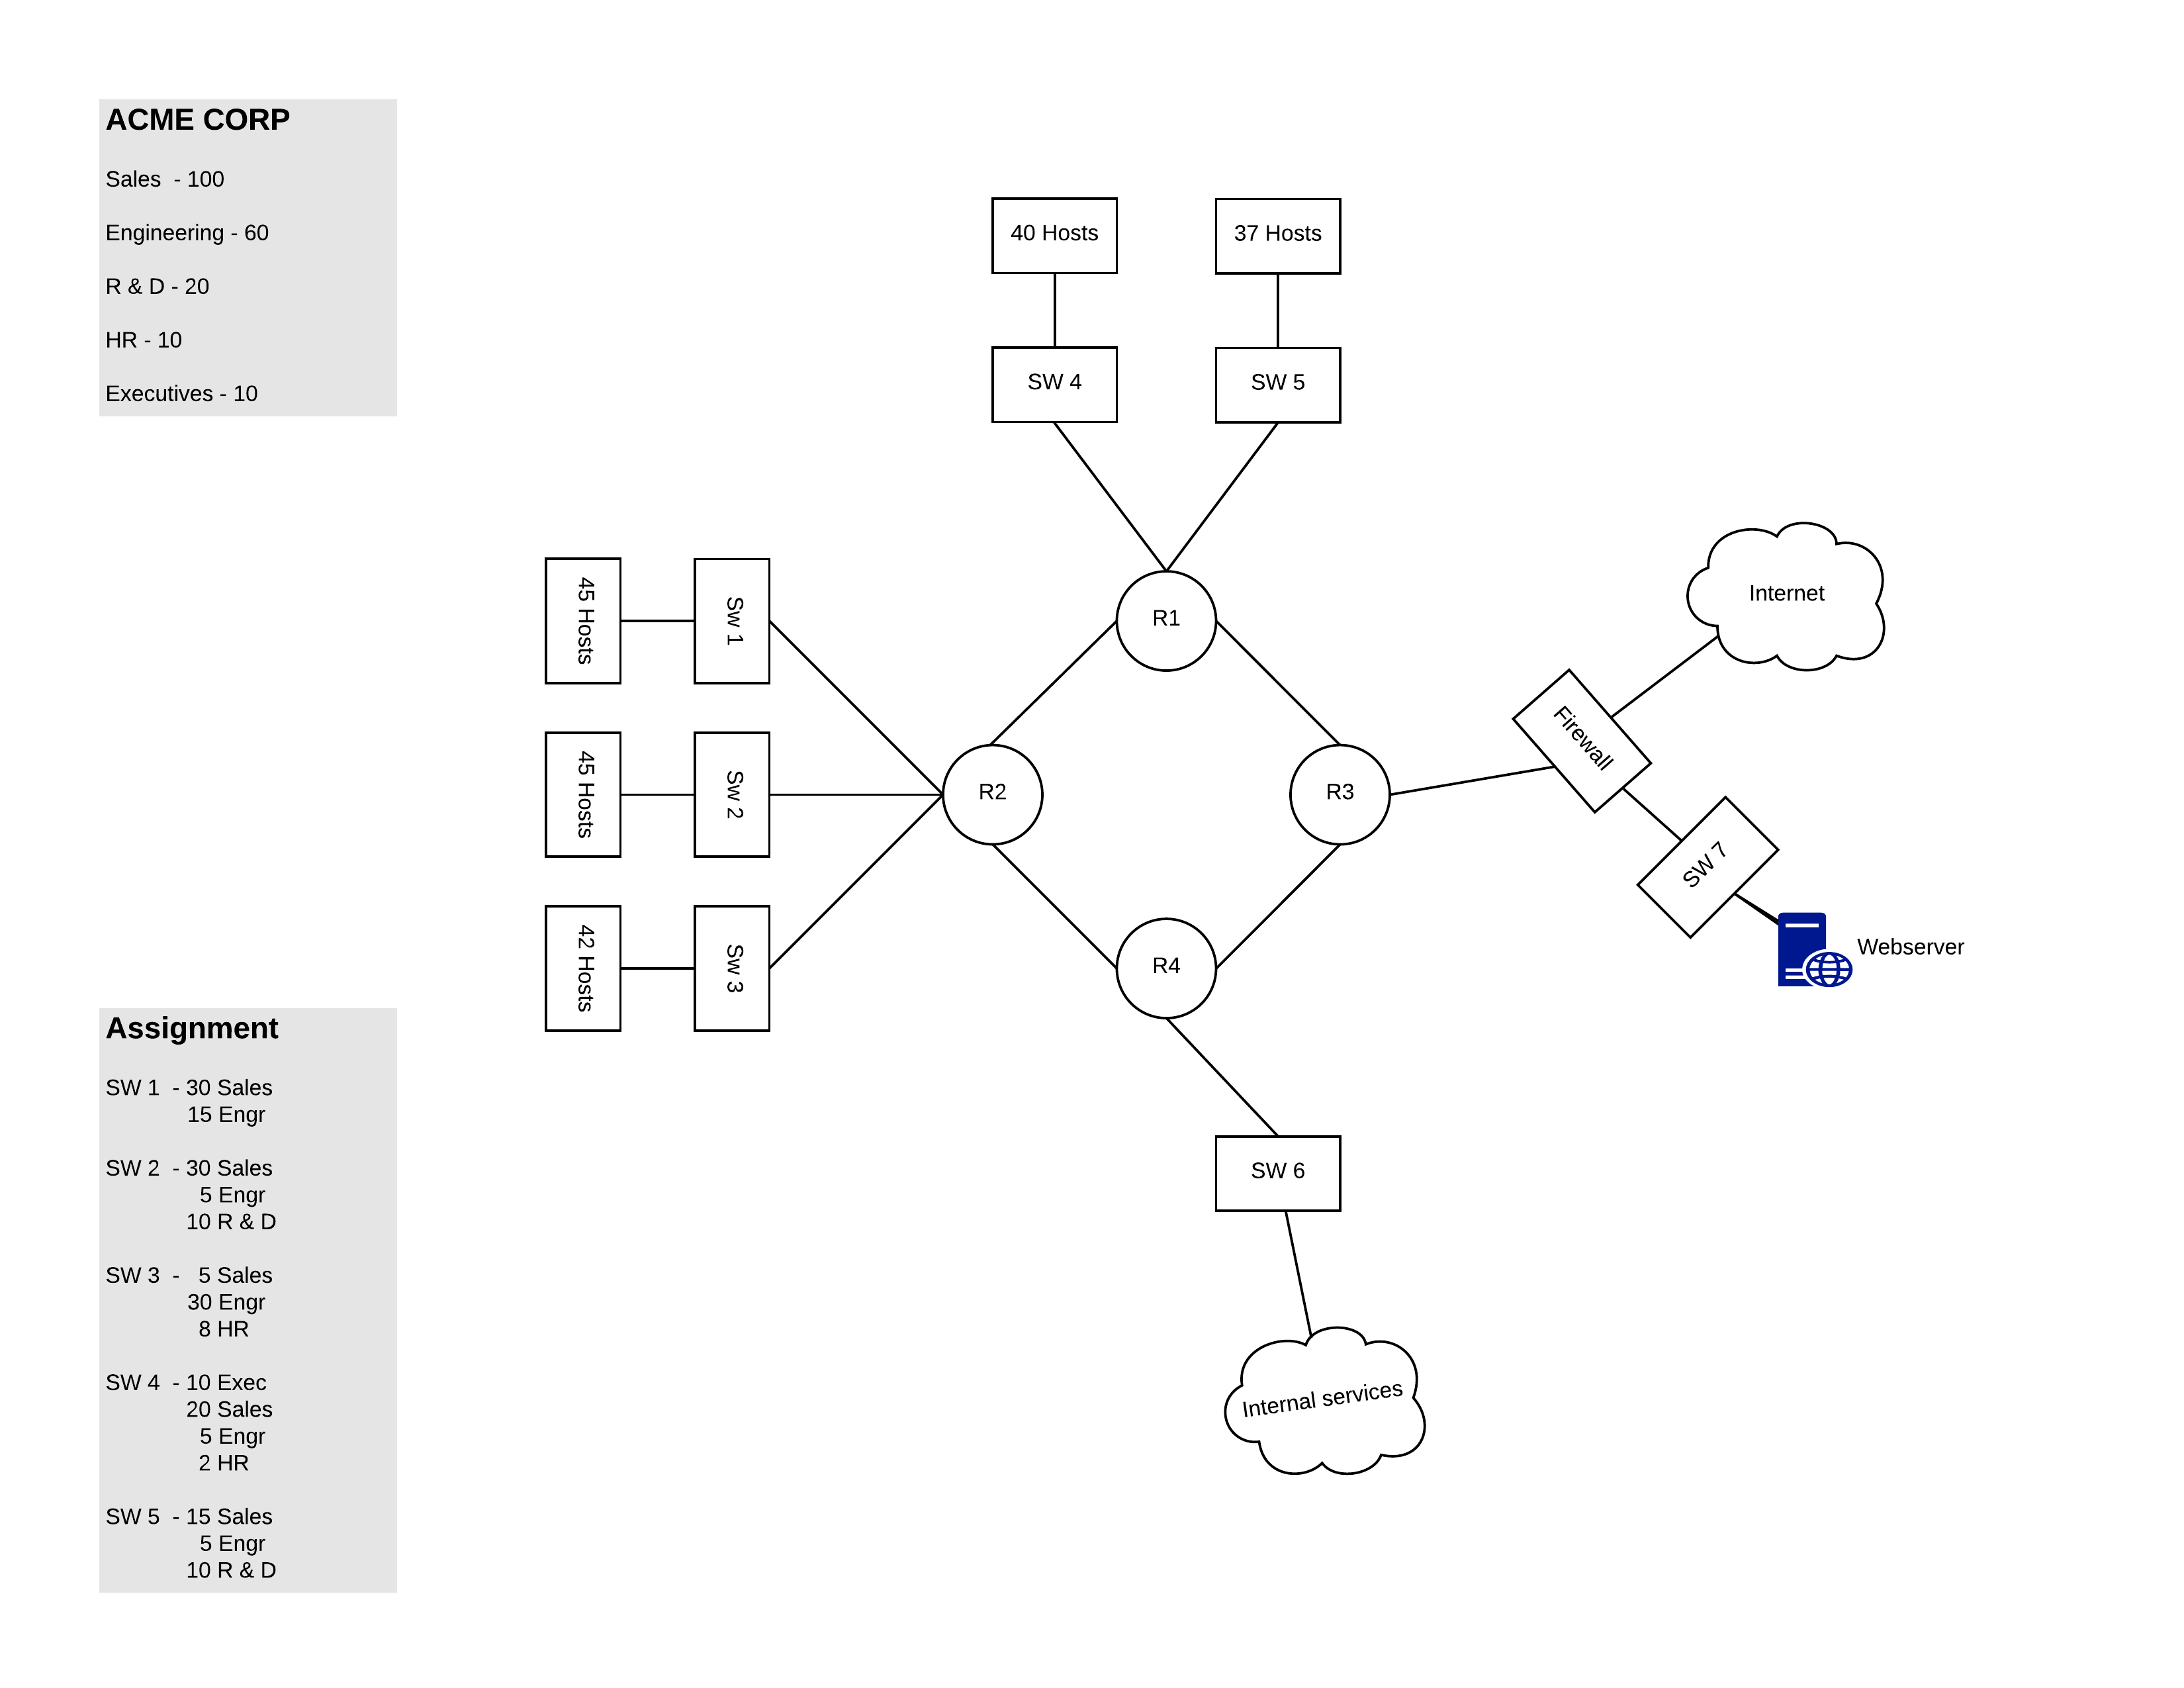
\includegraphics[width=\textwidth]{images/networktopology.png}
	\caption{Topology Map for Acme Corp}
\end{figure}
